\documentclass[a4paper,14pt]{extreport} % формат документа

\usepackage{amsmath}
\usepackage{cmap} % поиск в ПДФ
\usepackage[T2A]{fontenc} % кодировка
\usepackage[utf8]{inputenc} % кодировка исходного текста
\usepackage[english,russian]{babel} % локализация и переносы
\usepackage[left = 2cm, right = 1cm, top = 2cm, bottom = 2 cm]{geometry} % поля
\usepackage{listings}
\usepackage{graphicx} % для вставки рисунков
\usepackage{amsmath}
\usepackage{float}
\usepackage{longtable}
\usepackage{multirow}
\graphicspath{{pictures/}}
\DeclareGraphicsExtensions{.pdf,.png,.jpg}
\newcommand{\anonsection}[1]{\section*{#1}\addcontentsline{toc}{section}{#1}}

\lstset{ %
	language=Prolog,                % Язык программирования 
	numbers=left,                   % С какой стороны нумеровать          
	frame=single,                    % Добавить рамку
}

\begin{document}
\begin{titlepage}

    \begin{table}[H]
        \centering
        \footnotesize
        \begin{tabular}{cc}
            \multirow{8}{*}{
\includegraphics[scale=0.35]{bmstu.jpg}}
            & \\
            & \\
            & \textbf{Министерство науки и высшего образования Российской Федерации} \\
            & \textbf{Федеральное государственное бюджетное образовательное учреждение} \\
            & \textbf{высшего образования} \\
            & \textbf{<<Московский государственный технический} \\
            & \textbf{университет имени Н.Э. Баумана>>} \\
            & \textbf{(МГТУ им. Н.Э. Баумана)} \\
        \end{tabular}
    \end{table}

    \vspace{-2.5cm}

    \begin{flushleft}
        \rule[-1cm]{\textwidth}{3pt}
        \rule{\textwidth}{1pt}
    \end{flushleft}

    \begin{flushleft}
        \small
        ФАКУЛЬТЕТ
        \underline{<<Информатика и системы управления>>\ \ \ \ \ \ \ 
        \ \ \ \ \ \ \ \ \ \ \ \ \ \ \ \ \ \ \ \ \ \ \ \ \ \ \ \ \ \ \ 
    \ \ \ \ \ \ \ \ \ \ \ \ \ \ \ } \\
        КАФЕДРА
        \underline{<<Программное обеспечение ЭВМ и
        информационные технологии>>
        \ \ \ \ \ \ \ \ \ \ \ \ \ \ \ \ \ \ \ \ }
    \end{flushleft}

    \vspace{4cm}

    \begin{center}
        \textbf{Лабораторная работа № 16} \\ 
        \hfill
        
        \textbf{Использование правил в программе на Prolog} \\
        \vspace{0.5cm}
        \textbf{} \\
    \end{center}

    \vspace{4cm}

    \begin{flushleft}
        \begin{tabular}{ll}
            \textbf{Дисциплина} & Функциональное и логическое программирование \\
            \textbf{Студент} & Сиденко А.Г. \\
            \textbf{Группа} & ИУ7-63Б \\
            \textbf{Преподаватель} & Толпинская Н.Б., Строганов Ю.В.  \\
        \end{tabular}
    \end{flushleft}

    \vspace{4cm}

   \begin{center}
        Москва, 2020 г.
    \end{center}

\end{titlepage}

\textbf{Задание}

Создать базу знаний: <<ПРЕДКИ>>, позволяющую наиболее эффективным способом (за меньшее количество шагов, что обеспечивается меньшим количеством предложений БЗ - правил), используя разные варианты (примеры) одного вопроса, определить (указать: какой вопрос для какого варианта):
\begin{enumerate}
\item по имени субъекта определить всех его бабушек (предки 2-го колена),
\item по имени субъекта определить всех его дедушек (предки 2-го колена),
\item по имени субъекта определить всех его бабушек и дедушек (предки 2-го колена),
\item по имени субъекта определить его бабушку по материнской линии (предки 2-го колена),
\item по имени субъекта определить его бабушку и дедушку по материнской линии (предки 2-го колена).
\end{enumerate}

Минимизировать количество правил и количество вариантов вопросов. Использовать конъюнктивные правила и простой вопрос.

Для одного из вариантов вопроса и конкретной БЗ составить таблицу, отражающую конкретный порядок работы системы

\hfill

\textbf{Программа}

\begin{lstlisting}
domains
  name = symbol
        
predicates
  mother(name, name).
  father(name, name).
  grandfatherF(name, name).
  grandfatherM(name, name).
  grandmotherF(name, name).
  grandmotherM(name, name).
  allGrandmothers(name, name).
  allGrandfathers(name, name).
  allGrandparents(name, name).
  grandparentsM(name, name)

clauses
  mother(maria, ann).
  mother(maria, yulia).
  mother(irina, dima).
  mother(ann, petr).
  father(ivan, ann).
  father(ivan, yulia).
  father(maksim, dima).
  father(dima, petr).
  
  % Grandfather on the mother line
  grandfatherM(X, Y):- father(X, Z), mother(Z, Y).
  % Grandfather on the father line
  grandfatherF(X, Y):- father(X, Z), father(Z, Y).
  % Grandmother on the mother line
  grandmotherM(X, Y):- mother(X, Z), mother(Z, Y).
  % Grandmother on the father line
  grandmotherF(X, Y):- mother(X, Z), father(Z, Y).
  
  % All grandmothers
  allGrandmothers(X, Y):- grandmotherM(X, Y).
  allGrandmothers(X, Y):- grandmotherF(X, Y).
  
  % All grandfathers
  allGrandfathers(X, Y):- grandfatherM(X, Y).
  allGrandfathers(X, Y):- grandfatherF(X, Y).
  
  % All grandpsrents
  allGrandparents(X, Y):- allGrandfathers(X, Y).
  allGrandparents(X, Y):- allGrandmothers(X, Y).
  
  % Grandparents on the mother line
  grandparentsM(X, Y):- grandfatherM(X, Y).
  grandparentsM(X, Y):- grandmotherM(X, Y).
\end{lstlisting}

\textbf{Примеры работы:}

\begin{enumerate}
\item по имени субъекта определить всех его бабушек (предки 2-го колена),

\begin{lstlisting}
goal
  allGrandmothers(X, petr).
\end{lstlisting}

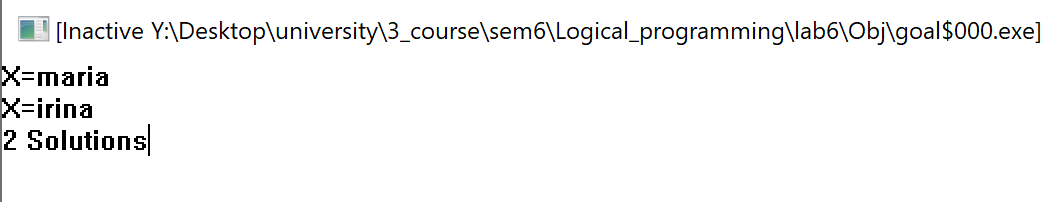
\includegraphics[scale=0.8]{ex1}

\item по имени субъекта определить всех его дедушек (предки 2-го колена),

\begin{lstlisting}
goal
  allGrandfathers(X, petr).
\end{lstlisting}

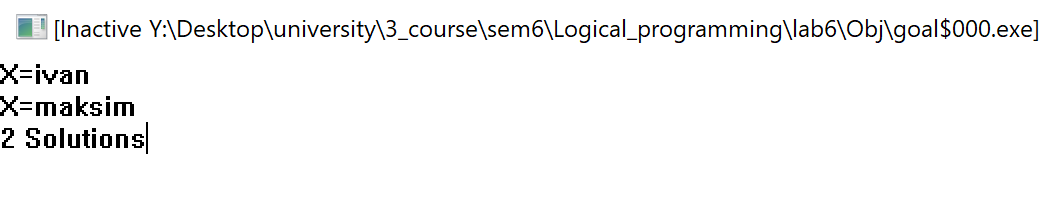
\includegraphics[scale=0.8]{ex2}

\item по имени субъекта определить всех его бабушек и дедушек (предки 2-го колена),

\begin{lstlisting}
goal
  allGrandparents(X, petr).
\end{lstlisting}

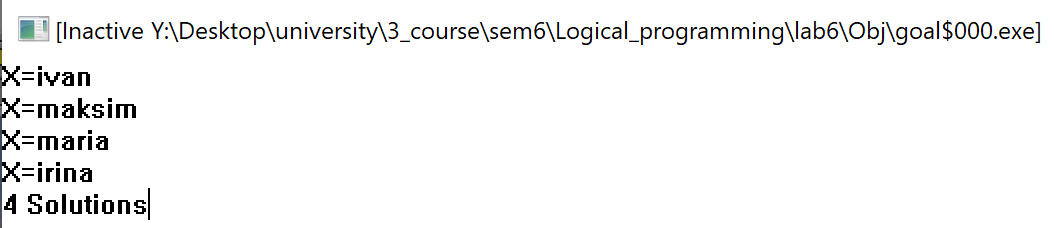
\includegraphics[scale=0.8]{ex3}

\item по имени субъекта определить его бабушку по материнской линии (предки 2-го колена),

\begin{lstlisting}
goal
  grandmotherM(X, petr).
\end{lstlisting}

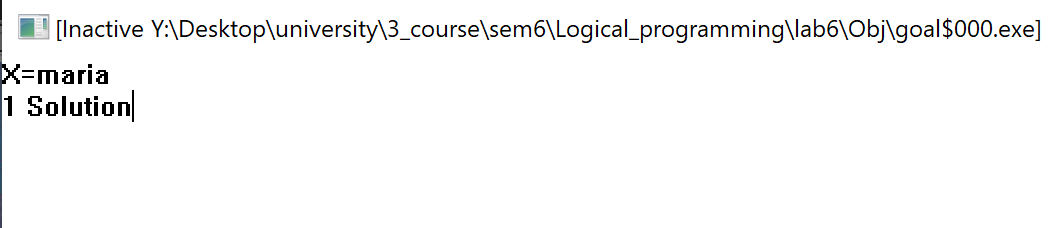
\includegraphics[scale=0.8]{ex4}

\item по имени субъекта определить его бабушку и дедушку по материнской линии (предки 2-го колена).

\begin{lstlisting}
goal
  grandparentsM(X, petr).
\end{lstlisting}

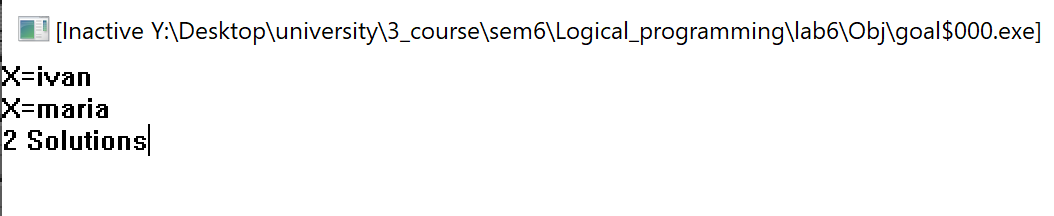
\includegraphics[scale=0.8]{ex5}

\end{enumerate}

\textbf{Приведем таблицу для задания 4. }

\begin{longtable}{|p{0.5cm}|p{4cm}|p{7cm}|p{5.5cm}|}
	\hline
 	№ шага & Состояние резольвенты & Сравниваемые термы; результат; подстановка, если есть  & Дальнейшие действия: прямой ход или откат \\ \hline
	1 & grandmotherM(X, petr) & По grandmotherM(X, petr) ищется системой определение отношения (по имени предиката и списку (числу) аргументов) & Определение отношения найдено, заносится в стек grandmotherM(X, petr), прямой ход \\ \hline
	2 &mother(X, Z), mother(Z, petr)& Начинает <<раскрываться>> правило, т.е. доказывается каждое целевое утверждение в теле правила последовательно слева направо
	mother(X, Z), mother(Z, petr)
	
	& Заносится в стек mother(X, Z)\\ \hline

	3 &mother(X, Z), mother(Z, petr)& По mother(X, Z)  ищется системой определение отношения (по имени предиката и списку (числу) аргументов) & Определение отношения найдено \\ \hline
	4 &mother(X, Z), mother(Z, petr)& Унификация mother(X, Z) с mother(maria, ann) & Результат сравнения термов: true, X примет значение maria, Z = ann. Установим маркер. Анонимные переменные не связываются со значением. Переход к следующему целевому утверждению в теле правила (прямой ход) \\ \hline
	5 & mother(ann, petr) & По mother(ann, petr)  ищется системой определение отношения (по имени предиката и списку (числу) аргументов) & Определение отношения найдено \\ \hline
	6 &mother(ann, petr) & Унификация mother(ann, petr) с mother(maria, ann) & Результат сравнения термов: false, переход к следующей строке (прямой ход) \\ \hline
	7 &mother(ann, petr) & Унификация mother(ann, petr) с mother(maria, yulia) & Результат сравнения термов: false, переход к следующей строке (прямой ход) \\ \hline
	8 &mother(ann, petr) & Унификация mother(ann, petr) с mother(irina, dima) & Результат сравнения термов: false, переход к следующей строке (прямой ход) \\ \hline
	9 &mother(ann, petr) & Унификация mother(ann, petr) с mother(ann, petr) & Результат сравнения термов: true. Установим маркер. Анонимные переменные не связываются со значением. Переход к следующему целевому утверждению в теле правила (прямой ход) \\ \hline
	10 &Резольвента пустая, успех&  &  В базе знаний больше ни одного утверждения с заданным именем, возврат, достаем из стека mother(ann, petr) \\ \hline
	11 &mother(X, Z), mother(Z, petr)& Унификация mother(X, Z) с mother(maria, yulia) & Результат сравнения термов: true, X примет значение maria, Z = yulia. Установим маркер. Анонимные переменные не связываются со значением. Переход к следующему целевому утверждению в теле правила (прямой ход) \\ \hline
	12 & mother(yulia, petr) & По mother(yulia, petr)  ищется системой определение отношения (по имени предиката и списку (числу) аргументов) & Определение отношения найдено \\ \hline
	13 &mother(yulia, petr) & Унификация mother(yulia, petr) с mother(maria, ann) & Результат сравнения термов: false, переход к следующей строке (прямой ход) \\ \hline
	14 &mother(yulia, petr) & Унификация mother(yulia, petr) с mother(maria, yulia) & Результат сравнения термов: false, переход к следующей строке (прямой ход) \\ \hline
	15 &mother(yulia, petr) & Унификация mother(yulia, petr) с mother(irina, dima) & Результат сравнения термов: false, переход к следующей строке (прямой ход) \\ \hline
	16 &mother(yulia, petr) & Унификация mother(yulia, petr) с mother(ann, petr) & Результат сравнения термов: false, В базе знаний больше ни одного утверждения с заданным именем, возврат, достаем из стека mother(yulia, petr) \\ \hline
	
	17 &mother(X, Z), mother(Z, petr)& Унификация mother(X, Z) с mother(irina, dima) & Результат сравнения термов: true, X примет значение irina, Z = dima. Установим маркер. Анонимные переменные не связываются со значением. Переход к следующему целевому утверждению в теле правила (прямой ход) \\ \hline
	18 & mother(dima, petr) & По mother(dima, petr)  ищется системой определение отношения (по имени предиката и списку (числу) аргументов) & Определение отношения найдено \\ \hline
	19 &mother(dima, petr) & Унификация mother(dima, petr) с mother(maria, ann) & Результат сравнения термов: false, переход к следующей строке (прямой ход) \\ \hline
	20 &mother(dima, petr) & Унификация mother(dima, petr) с mother(maria, yulia) & Результат сравнения термов: false, переход к следующей строке (прямой ход) \\ \hline
	21 &mother(dima, petr) & Унификация mother(dima, petr) с mother(irina, dima) & Результат сравнения термов: false, переход к следующей строке (прямой ход) \\ \hline
	22 &mother(dima, petr) & Унификация mother(dima, petr) с mother(ann, petr) & Результат сравнения термов: false, В базе знаний больше ни одного утверждения с заданным именем, возврат, достаем из стека mother(dima, petr) \\ \hline
	
	23 &mother(X, Z), mother(Z, petr)& Унификация mother(X, Z) с mother(ann, petr) & Результат сравнения термов: true, X примет значение ann, Z = petr. Установим маркер. Анонимные переменные не связываются со значением. Переход к следующему целевому утверждению в теле правила (прямой ход) \\ \hline
	24 & mother(petr, petr) & По mother(petr, petr)  ищется системой определение отношения (по имени предиката и списку (числу) аргументов) & Определение отношения найдено \\ \hline
	25 &mother(petr, petr) & Унификация mother(petr, petr) с mother(maria, ann) & Результат сравнения термов: false, переход к следующей строке (прямой ход) \\ \hline
	26 &mother(petr, petr) & Унификация mother(petr, petr) с mother(maria, yulia) & Результат сравнения термов: false, переход к следующей строке (прямой ход) \\ \hline
	27 &mother(petr, petr) & Унификация mother(petr, petr) с mother(irina, dima) & Результат сравнения термов: false, переход к следующей строке (прямой ход) \\ \hline
	28 &mother(petr, petr) & Унификация mother(petr, petr) с mother(ann, petr) & Результат сравнения термов: false, В базе знаний больше ни одного утверждения с заданным именем, возврат, достаем из стека mother(petr, petr) \\ \hline
	29 & &  Больше нет правил с заданным именем, достаем из стека grandmotherM(X, petr) & Стек пуст, завершение программы \\ \hline

\end{longtable}

\hfill

\textbf{Ответы на вопросы}

\begin{enumerate} 

\item В каком случае система запускает алгоритм унификации? (Как эту необходимость на формальном уровне распознает система?)

Пролог выполняет унификацию в двух случаях: когда цель сопоставляется с заголовком предложения или когда используется знак равенства, который является инфиксным предикатом (предикатом, который расположен между своими аргументами, а не перед ними).

\item Каковы назначение и результат использования алгоритма унификации? 

Унификация двух термов -- это основной шаг доказательства. В процессе работы система выполняет большое число унификаций.
\textbf{Унификация} -- операция, которая позволяет формализовать процесс логического вывода. 

Унификация представляет собой процесс сопоставления цели с фактами и правилами базы знаний. Цель может быть согласована, если она может быть сопоставлена с заголовком какого-либо предложения базы.

\item Какое первое состояние резольвенты?

Вопрос. 

\item Как меняется резольвента?

Резольвента - текущая цель, существующая на любой стадии вычислений. Резольвенты порождаются целью и каким-либо правилом или фактом, которые просматриваются последовательно сверху вниз. Если резольвента существует при наиболее общей унификации, она вычисляется. Если пустая резольвента с помощью такой стратегии не найдена, то ответ на вопрос отрицателен.

\item В каких пределах программы уникальны переменные? 

Областью действия переменной в Прологе является одно предложение. В разных предложениях может использоваться одно имя переменной для обозначения разных объектов. Исключением является анонимная переменная. Каждая анонимная переменная -- это отдельный объект.

\item Как применяется подстановка, полученная с помощью алгоритма унификации?

При согласовании переменные получают значения, указанные с другой стороны от знака <<=>>, если переменные еще не были связаны. Переменные становятся связанными и после успешного согласования всех целевых утверждений, будет напечатано значение связанных переменных.

\item В каких случаях запускается механизм отката?

Откат дает возможность получить много решений в одном вопросе к программе. 

Во всех точках программы, где существуют альтернативы, в стек заносятся точки возврата. 

Если впоследствии окажется, что выбранный вариант не приводит к успеху, то осуществляется откат к последней из имеющихся в стеке точек программы, где был выбран один из альтернативных вариантов. 

Выбирается очередной вариант, программа продолжает свою работу. Если все варианты в точке уже были использованы, то регистрируется неудачное завершение и осуществляется переход на предыдущую точку возврата, если такая есть. 

При откате все связанные переменные, которые были означены после этой точки, опять освобождаются.

\end{enumerate}
 
\end{document}